\UseRawInputEncoding
\documentclass[conference]{IEEEtran}
\IEEEoverridecommandlockouts

% ─── Idioma y codificación ───
\usepackage[spanish,es-noquoting]{babel}
\usepackage[utf8]{inputenc}
\usepackage[T1]{fontenc}

% ─── Matemáticas ───
\usepackage{amsmath,amssymb,amsfonts}

% ─── Figuras y tablas ───
\usepackage{graphicx}
\usepackage{booktabs,multirow,array}
\usepackage{float}

% ─── Algoritmos / pseudocódigo ───
\usepackage{algorithm}
\usepackage{algpseudocode}

% ─── TikZ ───
\usepackage{tikz}
\usetikzlibrary{shapes.geometric, arrows.meta, positioning, fit, calc, backgrounds, decorations.pathreplacing}
\tikzset{
  block/.style={rectangle, draw=black!70, fill=blue!8, thick,
                minimum width=2.0cm, minimum height=0.55cm,
                align=center, font=\scriptsize, rounded corners=2pt},
  qblock/.style={rectangle, draw=black!70, fill=purple!10, thick,
                 minimum width=2.0cm, minimum height=0.55cm,
                 align=center, font=\scriptsize, rounded corners=2pt},
  cblock/.style={rectangle, draw=black!70, fill=green!10, thick,
                 minimum width=2.0cm, minimum height=0.55cm,
                 align=center, font=\scriptsize, rounded corners=2pt},
  data/.style={trapezium, trapezium left angle=70, trapezium right angle=110,
               draw=black!70, fill=orange!12, minimum width=1.6cm,
               minimum height=0.45cm, align=center, font=\scriptsize},
  arrow/.style={-{Latex[length=2mm,width=1.5mm]}, thick, black!70},
  qgate/.style={rectangle, draw=black, fill=blue!15, minimum width=0.45cm,
                minimum height=0.45cm, font=\scriptsize, inner sep=1pt},
  qgateZ/.style={rectangle, draw=black, fill=purple!15, minimum width=0.45cm,
                 minimum height=0.45cm, font=\scriptsize, inner sep=1pt},
  qgateY/.style={rectangle, draw=black, fill=green!15, minimum width=0.45cm,
                 minimum height=0.45cm, font=\scriptsize, inner sep=1pt},
}

% ─── Hipervínculos ───
\usepackage[breaklinks, colorlinks=true, linkcolor=black, citecolor=blue!60!black, urlcolor=blue!70!black]{hyperref}

\def\BibTeX{{\rm B\kern-.05em{\sc i\kern-.025em b}\kern-.08em
    T\kern-.1667em\lower.7ex\hbox{E}\kern-.125emX}}

\begin{document}

\title{Descomposición de la Escasez Muestral y el Ruido NISQ en la Clasificación de Kernel Cuántico: un Protocolo Empírico bajo Restricciones de Acceso en IBM Heron r2\\
\thanks{\raisebox{-9pt}{
\includegraphics[height=26pt]{graficos/escudo.png}}\ \ Trabajo desarrollado en el curso de Computación Cuántica, Escuela Profesional de Ingeniería Informática y de Sistemas, Universidad Nacional de San Antonio Abad del Cusco (UNSAAC).}}

\author{
\IEEEauthorblockN{Edmil Jampier Saire Bustamante}
\IEEEauthorblockA{
\textit{Escuela Profesional de Ingeniería Informática y de Sistemas}\\
\textit{Universidad Nacional de San Antonio Abad del Cusco}\\
Cusco, Perú \\
174449@unsaac.edu.pe}
\and
\IEEEauthorblockN{Medaly Lozano Llacctahuaman}
\IEEEauthorblockA{
\textit{Escuela Profesional de Ingeniería Informática y de Sistemas}\\
\textit{Universidad Nacional de San Antonio Abad del Cusco}\\
Cusco, Perú \\
195040@unsaac.edu.pe}
\and
\IEEEauthorblockN{José Francisco Puma Potosino}
\IEEEauthorblockA{
\textit{Escuela Profesional de Ingeniería Informática y de Sistemas}\\
\textit{Universidad Nacional de San Antonio Abad del Cusco}\\
Cusco, Perú \\
164248@unsaac.edu.pe}
}

\maketitle

\begin{abstract}
La degradación de clasificadores cuánticos en hardware NISQ suele reportarse como un único valor de exactitud, atribuido genéricamente al ruido, sin distinguir cuánto proviene de la escasez de datos impuesta por las cuotas de acceso gratuito y cuánto del ruido físico del procesador. Este trabajo propone y valida un protocolo de descomposición de tres puntos que aísla ambas causas sobre una Máquina de Vectores de Soporte Cuántica (QSVC) con kernel de fidelidad ZZFeatureMap, evaluada sobre el conjunto de datos Iris: (1) simulador ideal con el conjunto completo, (2) simulador ideal sobre el mismo subconjunto reducido usado en hardware, y (3) el procesador real \texttt{ibm\_fez} de IBM (Heron r2, 156 qubits) sobre ese subconjunto. La cadena de mediciones aisló un efecto puro de escasez muestral de $-$44 puntos porcentuales (de 77.78\,\% a 33.33\,\%) y un efecto puro adicional de ruido de hardware de $-$22 puntos porcentuales (hasta 11.11\,\%). Se verificó la calidad del hardware mediante la fidelidad del estado de Bell (0.9834) y se evaluó la mitigación de lectura TREX, que no revirtió la degradación, lo que sugiere daño acumulado a nivel de compuerta más que de lectura. Se documentó además un caso en que el hardware superó al simulador en una tarea binaria (MNIST, 88.89\,\% frente a 77.78\,\%), identificado como artefacto estadístico de baja resolución muestral y no como evidencia de ventaja cuántica. Se concluye que el protocolo de descomposición propuesto ofrece un método reproducible para atribuir causas de degradación en QML bajo las restricciones reales del acceso gratuito a hardware cuántico, complementado con un clasificador variacional (VQC) y baselines clásicos (SVM-RBF, MLP, KNN) como marco de referencia.
\end{abstract}

\begin{IEEEkeywords}
Quantum Machine Learning, Quantum Kernel Methods, NISQ, Error Mitigation, Reproducibility, IBM Quantum
\end{IEEEkeywords}

\section{Introducción}
\label{sec:introduccion}

Durante la etapa computacional conocida como \textit{Noisy Intermediate-Scale Quantum} (NISQ), los algoritmos híbridos cuántico-clásicos de aprendizaje automático cuántico (\textit{Quantum Machine Learning}, QML) se presentan como los candidatos más viables para explorar una eventual ventaja computacional cuántica \cite{preskill2018}. Estos modelos explotan la superposición y el entrelazamiento \cite{biamonte2017} para mapear datos clásicos a espacios de Hilbert de alta dimensionalidad, con la expectativa de que dicho mapeo capture correlaciones difíciles de representar clásicamente \cite{havlicek2019}.

El problema que motiva este trabajo es metodológico: la gran mayoría de los estudios que ejecutan QML en hardware real reportan un único número de \textit{accuracy} y lo atribuyen genéricamente ``al ruido'', sin descomponerlo en sus causas. Esto es particularmente problemático bajo el régimen de acceso gratuito a la nube de IBM Quantum (10 minutos de QPU mensuales), que obliga a trabajar con muestras extremadamente reducidas. En ese régimen, la escasez de datos y el ruido físico del procesador operan simultáneamente sobre el mismo experimento, y sin un diseño que los separe no es posible determinar si una técnica de mitigación de errores es realmente inefectiva o si simplemente opera sobre datos insuficientes para generalizar.

Este trabajo propone un \textbf{protocolo de descomposición de tres puntos}: se mide el mismo clasificador de kernel cuántico (QSVC) primero sobre el conjunto de datos completo en simulador ideal, luego sobre el subconjunto reducido en simulador ideal, y finalmente sobre ese mismo subconjunto en el procesador físico \texttt{ibm\_fez}. Al mantener fijos el kernel, el subconjunto y el modelo clásico downstream, y variar únicamente el entorno de ejecución entre pasos consecutivos, la caída de \textit{accuracy} en cada paso puede atribuirse a una causa específica: el primer salto aísla el efecto de la escasez muestral y el segundo aísla el efecto del ruido de hardware. Esto contrasta con los \textit{benchmarks} a gran escala existentes, centrados en comparaciones agregadas simulador-clásico sobre datasets completos \cite{bowles2024,schnabel2024}, que no reportan esta descomposición causal en el régimen de tamaños muestrales impuesto por el acceso gratuito a hardware real.

Las contribuciones de este artículo son: (i) un \textbf{protocolo reproducible de descomposición cuantitativa} muestra-vs-ruido, validado empíricamente con una caída de $-$44 puntos porcentuales por escasez muestral y $-$22 puntos porcentuales adicionales por ruido de hardware sobre la misma QSVC; (ii) la \textbf{caracterización del mecanismo de fallo} de la mitigación de lectura TREX sobre un kernel ya colapsado, contrastando la alta fidelidad de entrelazamiento básico del hardware (0.9834 en el estado de Bell) con su incapacidad para revertir la degradación del kernel, lo que sugiere que el daño ocurre a nivel de compuerta y no de lectura; y (iii) la \textbf{documentación de un artefacto de reproducibilidad} bajo el tier gratuito: la aparente superioridad del hardware sobre el simulador en una tarea binaria (MNIST) se explica por la baja resolución estadística de 9 muestras de prueba y no por ventaja cuántica, una advertencia relevante para quienes trabajan con las mismas restricciones de acceso.

El resto del artículo se organiza como sigue: la Sección~\ref{sec:related} revisa trabajos relacionados y señala explícitamente el vacío que este protocolo llena; la Sección~\ref{sec:teoria} presenta el marco teórico; la Sección~\ref{sec:metodologia} describe el protocolo de descomposición y la arquitectura del sistema; la Sección~\ref{sec:implementacion} detalla la implementación y el repositorio; la Sección~\ref{sec:experimentacion} describe el diseño experimental; la Sección~\ref{sec:resultados} presenta los resultados organizados alrededor de la cadena de descomposición; la Sección~\ref{sec:discusion} los discute críticamente; y la Sección~\ref{sec:conclusiones} concluye con el trabajo futuro.

\section{Trabajos Relacionados}
\label{sec:related}

\subsection{Fundamentos y benchmarking crítico de QML}
Los cimientos formales del QML fueron establecidos por Biamonte \textit{et al.} \cite{biamonte2017}, quienes sistematizan cómo la superposición y el entrelazamiento pueden acelerar tareas de aprendizaje. Havlíček \textit{et al.} \cite{havlicek2019} introducen el VQC y el kernel de fidelidad cuántica evaluados en hardware IBM temprano, y Rebentrost \textit{et al.} \cite{rebentrost2014} formulan la QSVM bajo supuestos de acceso a memoria cuántica (QRAM) poco realistas en el hardware NISQ actual. Trabajos más recientes adoptan una postura crítica frente a este optimismo inicial: Bowles \textit{et al.} \cite{bowles2024} realizan un \textit{benchmark} a gran escala sobre 12 modelos cuánticos y 160 conjuntos de datos, concluyendo que los clasificadores clásicos \textit{fuera de la caja} superan sistemáticamente a los cuánticos; Schnabel \textit{et al.} \cite{schnabel2024} comparan \textit{Fidelity Quantum Kernels} y \textit{Projected Quantum Kernels}, mostrando que el ancho de banda del kernel es determinante para la generalización. \textbf{Lo que falta:} ambos \textit{benchmarks} operan sobre datasets completos y reportan un valor agregado de degradación; ninguno aísla, dentro del mismo experimento, cuánto de esa degradación proviene de la cantidad de datos disponible frente al ruido físico del hardware.

\subsection{Teoría del fallo de kernels y circuitos variacionales}
En el plano teórico, McClean \textit{et al.} \cite{mcclean2018} y la síntesis posterior de Larocca \textit{et al.} \cite{larocca2025} caracterizan los \textit{barren plateaus} que dificultan el entrenamiento variacional, mientras que Thanasilp \textit{et al.} \cite{thanasilp2024} formalizan la \textbf{concentración exponencial}, un fenómeno análogo que degrada los kernels cuánticos al aumentar el número de qubits. Schuld y Killoran \cite{schuld2019} formalizan la interpretación de los \textit{feature maps} cuánticos como funciones de kernel en espacios de Hilbert, y Yu \textit{et al.} \cite{yu2025} sintetizan en una revisión reciente los algoritmos QML basados en circuitos variacionales, sin llegar a un consenso sobre condiciones de aplicabilidad práctica bajo ruido real. \textbf{Lo que falta:} estos trabajos explican matemáticamente \emph{por qué} un kernel cuántico puede colapsar, pero no ofrecen evidencia empírica de cómo ese colapso interactúa con una técnica de mitigación de errores concreta desplegada en hardware real.

\subsection{Poder de los datos y mitigación de errores}
Huang \textit{et al.} \cite{huang2021} establecen criterios formales sobre cuándo un conjunto de datos permite esperar ventaja cuántica genuina, un criterio que motiva directamente nuestra decisión de aislar el efecto muestral como variable independiente. En mitigación de errores, van den Berg \textit{et al.} \cite{vandenberg2022} formalizan la técnica de \textit{twirled readout error extinction} (TREX) con cotas de error aplicables para corregir asimetrías de lectura, mientras que Temme \textit{et al.} \cite{temme2017} proponen \textit{Zero Noise Extrapolation} (ZNE) para mitigar ruido a nivel de compuerta mediante extrapolación. \textbf{Lo que falta:} la literatura de mitigación de errores rara vez estudia el régimen en que TREX \emph{falla}, y menos aún sobre kernels cuánticos de fidelidad específicamente degradados por escasez muestral.

\subsection{Posicionamiento de esta contribución}
A diferencia de los estudios anteriores, que evalúan predominantemente en simuladores o en hardware con datasets completos, o que estudian el fallo de kernels y la mitigación de errores por separado, el presente trabajo ejecuta el kernel cuántico directamente sobre un procesador Heron r2 (\texttt{ibm\_fez}) bajo las restricciones reales de una cuota gratuita, descompone explícitamente la degradación observada en sus dos componentes causales (muestra y ruido) mediante un protocolo reproducible de tres puntos, y caracteriza el mecanismo por el cual una técnica de mitigación de errores concreta (TREX) resulta insuficiente en ese régimen --una combinación de condiciones no cubierta directamente por los trabajos citados.

\section{Marco Teórico}
\label{sec:teoria}

\subsection{Qubits, puertas y circuitos parametrizados}
El qubit es la unidad fundamental de información cuántica \cite{nielsen2010}. A diferencia del bit clásico, puede existir en superposición de los estados $|0\rangle$ y $|1\rangle$:
\begin{equation}
|\psi\rangle = \alpha|0\rangle + \beta|1\rangle, \quad |\alpha|^2+|\beta|^2=1,
\end{equation}
con $\alpha,\beta\in\mathbb{C}$. Un sistema de $n$ qubits vive en un espacio de Hilbert de dimensión $2^n$. Las puertas de rotación $R_Y(\theta)$ y $R_Z(\theta)$ permiten la codificación angular de datos clásicos, y las puertas $\mathrm{CNOT}$ generan entrelazamiento entre qubits, recurso esencial para capturar correlaciones no triviales \cite{nielsen2010}.

Un circuito parametrizado $U(\mathbf{x},\boldsymbol{\theta})$ combina un \textit{feature map} $U_\phi(\mathbf{x})$, que codifica datos clásicos en un estado cuántico, con un \textit{ansatz} $U_W(\boldsymbol{\theta})$ de parámetros entrenables. La Figura~\ref{fig:circuito} esquematiza esta arquitectura para el caso de 4 qubits utilizado en este trabajo; las Figuras~\ref{fig:zzfm_real} y~\ref{fig:vqc_real} muestran los circuitos reales generados por Qiskit, descompuestos en puertas básicas.

\begin{figure}[t]
\centering
\resizebox{\columnwidth}{!}{%
\begin{tikzpicture}[x=0.55cm, y=0.55cm]
  \foreach \q/\y in {0/0, 1/-1, 2/-2, 3/-3} {
    \node[font=\scriptsize] at (-0.6, \y) {$|0\rangle_{\q}$};
    \draw[thick] (-0.1, \y) -- (12.5, \y);
  }
  \foreach \q/\y in {0/0, 1/-1, 2/-2, 3/-3} {
    \node[qgate, fill=cyan!20] at (0.7, \y) {H};
    \node[qgateZ] at (1.7, \y) {\scriptsize $R_Z(x_{\q})$};
  }
  \foreach \q/\y in {0/0, 1/-1, 2/-2} {
    \pgfmathsetmacro\yn{\y - 1}
    \draw[thick] (3.2, \y) -- (3.2, \yn);
    \fill (3.2, \y) circle (1.5pt);
    \draw (3.2, \yn) circle (4pt);
  }
  \foreach \q/\y in {0/0, 1/-1, 2/-2} {
    \pgfmathsetmacro\yn{\y - 1}
    \draw[thick] (4.5, \y) -- (4.5, \yn);
    \fill (4.5, \y) circle (1.5pt);
    \draw (4.5, \yn) circle (4pt);
  }
  \foreach \q/\y in {0/0, 1/-1, 2/-2, 3/-3} {
    \node[qgateY] at (5.8, \y) {\scriptsize $R_Y(\theta)$};
  }
  \foreach \q/\y in {0/0, 1/-1, 2/-2} {
    \pgfmathsetmacro\yn{\y - 1}
    \draw[thick] (7.0, \y) -- (7.0, \yn);
    \fill (7.0, \y) circle (1.5pt);
    \draw (7.0, \yn) circle (4pt);
  }
  \foreach \q/\y in {0/0, 1/-1, 2/-2, 3/-3} {
    \node[qgateY] at (8.0, \y) {\scriptsize $R_Y(\theta)$};
  }
  \foreach \q/\y in {0/0, 1/-1, 2/-2} {
    \pgfmathsetmacro\yn{\y - 1}
    \draw[thick] (9.2, \y) -- (9.2, \yn);
    \fill (9.2, \y) circle (1.5pt);
    \draw (9.2, \yn) circle (4pt);
  }
  \foreach \q/\y in {0/0, 1/-1, 2/-2, 3/-3} {
    \node[qgate, fill=gray!25] at (10.7, \y) {\scriptsize M};
    \draw[thick, double, double distance=1pt] (10.95, \y) -- (12.5, \y);
  }
  \draw[decorate,decoration={brace,amplitude=4pt}]
    (0.3, 0.7) -- (4.8, 0.7) node[midway,above=2pt,font=\scriptsize\bfseries]
    {Feature map $U_\phi(\mathbf{x})$};
  \draw[decorate,decoration={brace,amplitude=4pt}]
    (5.3, 0.7) -- (9.6, 0.7) node[midway,above=2pt,font=\scriptsize\bfseries]
    {Ansatz $U_W(\boldsymbol{\theta})$};
  \draw[decorate,decoration={brace,amplitude=4pt}]
    (10.2, 0.7) -- (12.3, 0.7) node[midway,above=2pt,font=\scriptsize\bfseries]
    {Medición};
\end{tikzpicture}%
}
\caption{Arquitectura del circuito cuántico de 4 qubits: ZZFeatureMap (codificación angular + entrelazamiento lineal) seguido del \textit{ansatz} RealAmplitudes y medición en la base computacional.}
\label{fig:circuito}
\end{figure}

\begin{figure}[t]
    \centering
    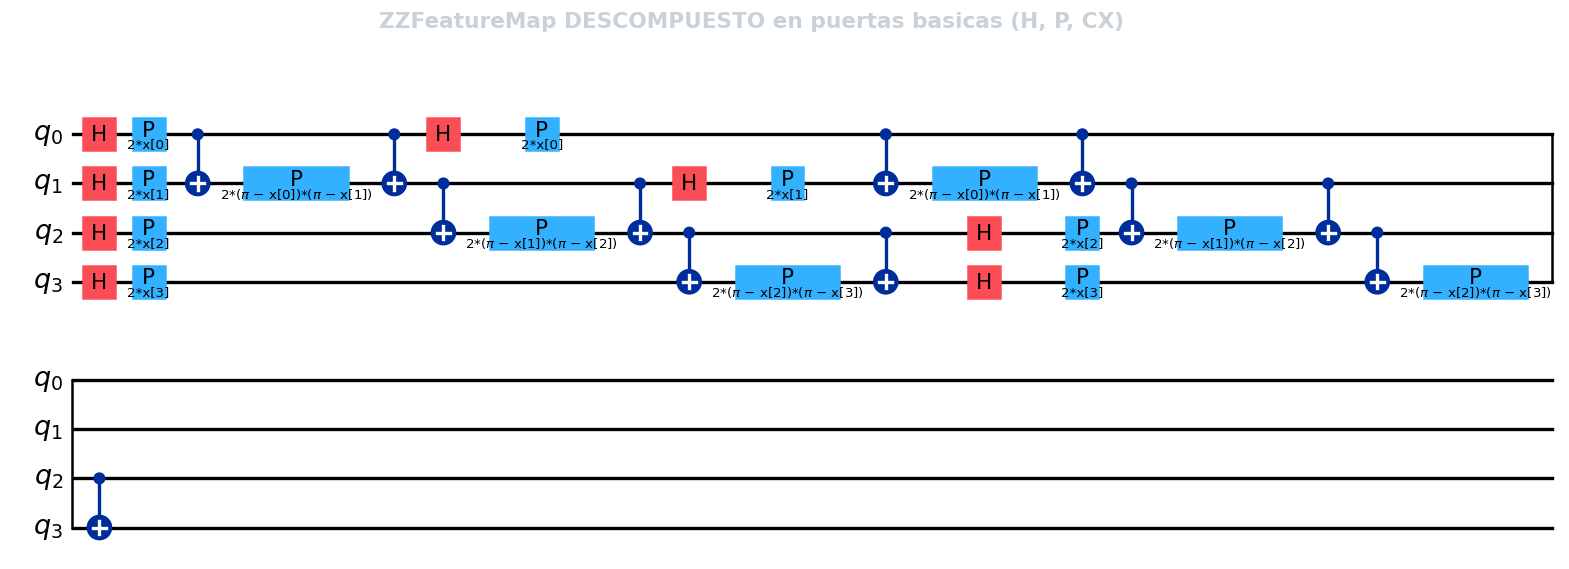
\includegraphics[width=\linewidth]{graficos/vis3_zzfeaturemap_2.png}
    \caption{ZZFeatureMap real descompuesto en puertas básicas (H, P, CX): 4 qubits, 2 repeticiones, entrelazamiento lineal. Cada repetición codifica las 4 características como fases $P(2x_i)$ y sus interacciones ZZ mediante pares CNOT-P-CNOT entre qubits vecinos.}
    \label{fig:zzfm_real}
\end{figure}

\begin{figure}[t]
    \centering
    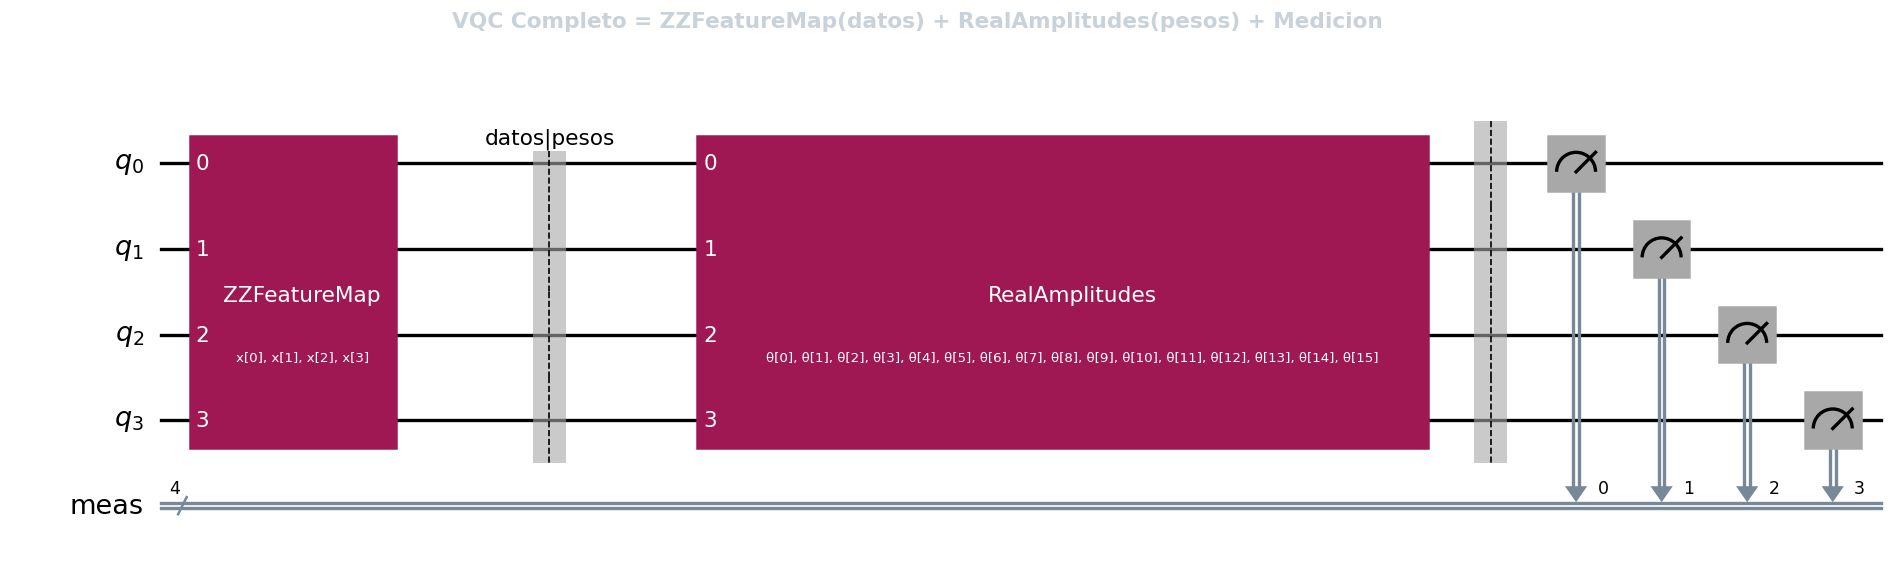
\includegraphics[width=\linewidth]{graficos/vis4_realamplitudes_vqc_2.png}
    \caption{Ansatz RealAmplitudes (16 parámetros entrenables, reps=3) y circuito VQC completo: ZZFeatureMap $+$ barrera $+$ RealAmplitudes $+$ medición. Flujo: $|0000\rangle \to U_\phi(\mathbf{x}) \to U_W(\boldsymbol{\theta}) \to$ Medición.}
    \label{fig:vqc_real}
\end{figure}

\subsection{VQC y QSVC}
El VQC \cite{havlicek2019} entrena de forma híbrida los parámetros $\boldsymbol{\theta}$ minimizando la entropía cruzada
\begin{equation}
\mathcal{L}(\boldsymbol{\theta}) = -\frac{1}{N}\sum_{i=1}^{N}\sum_{c=1}^{C} y_{ic}\,\log\!\left(\hat{y}_{ic}(\boldsymbol{\theta})\right),
\end{equation}
mientras un optimizador clásico (COBYLA, SPSA o L-BFGS-B) actualiza $\boldsymbol{\theta}$ entre evaluaciones del circuito cuántico \cite{cerezo2021}. La QSVC \cite{rebentrost2014,havlicek2019} sustituye el kernel clásico por un kernel de fidelidad
\begin{equation}
K_Q(\mathbf{x}_i,\mathbf{x}_j) = \left|\langle\phi(\mathbf{x}_j)|\phi(\mathbf{x}_i)\rangle\right|^2,
\end{equation}
con $|\phi(\mathbf{x})\rangle = U_\phi(\mathbf{x})|0\rangle^{\otimes n}$, y delega la optimización cuadrática a un SVC clásico \cite{schuld2019}. El SVM-RBF clásico, utilizado como \textit{baseline}, emplea el kernel $K(\mathbf{x}_i,\mathbf{x}_j)=\exp(-\gamma\|\mathbf{x}_i-\mathbf{x}_j\|^2)$.

Los circuitos profundos pueden sufrir \textit{barren plateaus} \cite{mcclean2018,larocca2025}, regiones donde los gradientes se desvanecen exponencialmente con el número de qubits; los kernels cuánticos sufren un fenómeno análogo de \textbf{concentración exponencial} \cite{thanasilp2024}, donde sus valores se vuelven indistinguibles al aumentar la dimensionalidad. Este resultado teórico es la base de la hipótesis mecanística discutida en la Sección~\ref{sec:discusion}: un kernel ya afectado por concentración exponencial y escasez de datos no puede recuperarse mediante correcciones de lectura.

\subsection{Fidelidad del estado de Bell}
El estado $|\Phi^+\rangle=\frac{1}{\sqrt{2}}(|00\rangle+|11\rangle)$ es el patrón métrico estándar para validar hardware cuántico: idealmente converge a $P(00){=}P(11){=}0.5$, y su desviación experimental cuantifica el ruido combinado de preparación, compuerta $CX$ y medición (\textit{SPAM errors}). Se utiliza en este trabajo como control independiente de la calidad del hardware, separado del experimento principal de degradación del kernel.

\subsection{Mitigación de errores: TREX y ZNE}
\textit{Twirled Readout Error Extinction} (TREX) \cite{vandenberg2022} aplica compuertas Pauli-X aleatorias antes de la medición y deshace su efecto en post-procesamiento clásico, trasladando el ruido de lectura asimétrico a un canal de depolarización local, sin necesidad de aumentar la profundidad del circuito principal. Por diseño, TREX corrige exclusivamente errores de medición (SPAM); no actúa sobre el ruido acumulado durante la ejecución de las puertas del circuito. \textit{Zero Noise Extrapolation} (ZNE) \cite{temme2017}, en cambio, opera sobre el ruido de compuerta amplificando artificialmente el ruido del circuito en varios niveles y extrapolando al límite de ruido cero, por lo que constituye una alternativa natural cuando la degradación no proviene de la lectura.

\section{Metodología}
\label{sec:metodologia}

La investigación es de tipo \textbf{experimental y comparativa}, articulada alrededor del \textbf{protocolo de descomposición de tres puntos} descrito en la Sección~\ref{sec:introduccion}: se implementan modelos cuánticos (VQC, QSVC) y clásicos (SVM-RBF, MLP, KNN) bajo condiciones controladas, y se mide el mismo clasificador de kernel cuántico en tres entornos progresivos --simulador con dataset completo, simulador con subconjunto reducido, hardware real con ese mismo subconjunto-- manteniendo fijos el kernel, los datos y el modelo downstream para que la diferencia entre pasos consecutivos sea atribuible a una única causa. La arquitectura del sistema comprende cuatro módulos (Figura~\ref{fig:pipeline}): (i) un módulo de entrada que gestiona carga, PCA y codificación angular; (ii) un módulo de procesamiento clásico (optimizador COBYLA para VQC, SVC dual para QSVC); (iii) un módulo de procesamiento cuántico que evalúa el kernel de fidelidad mediante la primitiva \texttt{SamplerV2}; y (iv) un módulo de salida para métricas e histogramas.

\begin{figure*}[t]
\centering
\resizebox{\textwidth}{!}{%
\begin{tikzpicture}[node distance=0.45cm and 0.6cm]
  \node[data] (ds) {Dataset (Iris / MNIST)};
  \node[block, right=of ds] (pp) {Preprocesamiento\\Normalización $[0,\pi]$ + PCA};
  \node[block, right=of pp] (sp) {\textit{Split} 70/30\\(estratificado)};
  \node[qblock, above right=0.3cm and 0.7cm of sp] (qfm) {\textit{Feature map}\\ZZFeatureMap};
  \node[qblock, right=of qfm] (qan) {\textit{Ansatz}\\RealAmplitudes};
  \node[qblock, right=of qan] (qopt) {Optimizador\\COBYLA (VQC)};
  \node[qblock, right=of qopt] (qpred) {VQC / QSVC\\(sim. o \texttt{ibm\_fez})};
  \node[cblock, below right=0.3cm and 0.7cm of sp] (csvm) {SVM-RBF};
  \node[cblock, right=of csvm] (cmlp) {MLP};
  \node[cblock, right=of cmlp] (cknn) {KNN};
  \node[cblock, right=of cknn] (cpred) {\textit{Baseline}\\predicción};
  \node[block, fill=yellow!15, right=0.7cm of $(qpred)!0.5!(cpred)$] (eval)
        {Métricas:\\\textit{accuracy}, P, R, F1\\Matriz confusión, tiempo};
  \node[data, fill=red!10, right=of eval] (out) {Análisis\\comparativo};
  \draw[arrow] (ds) -- (pp);
  \draw[arrow] (pp) -- (sp);
  \draw[arrow] (sp.east) -- ++(0.25,0) |- (qfm.west);
  \draw[arrow] (sp.east) -- ++(0.25,0) |- (csvm.west);
  \draw[arrow] (qfm) -- (qan);
  \draw[arrow] (qan) -- (qopt);
  \draw[arrow] (qopt) -- (qpred);
  \draw[arrow] (csvm) -- (cmlp);
  \draw[arrow] (cmlp) -- (cknn);
  \draw[arrow] (cknn) -- (cpred);
  \draw[arrow] (qpred.east) -| (eval.north);
  \draw[arrow] (cpred.east) -| (eval.south);
  \draw[arrow] (eval) -- (out);
  \node[font=\scriptsize\bfseries, purple!70!black] at ([yshift=0.35cm]qan.north) {Rama cuántica};
  \node[font=\scriptsize\bfseries, green!50!black] at ([yshift=-0.35cm]cmlp.south) {Rama clásica};
\end{tikzpicture}%
}
\caption{Pipeline metodológico: la rama cuántica (arriba) y la clásica (abajo) parten del mismo preprocesamiento y convergen en una etapa de evaluación comparativa común.}
\label{fig:pipeline}
\end{figure*}

El Algoritmo~\ref{alg:pipeline} resume el procedimiento seguido para cada punto de la cadena de descomposición.

\begin{algorithm}[t]
\caption{Protocolo de descomposición de tres puntos (VQC/QSVC vs. clásicos)}
\label{alg:pipeline}
\begin{algorithmic}[1]
\State \textbf{Entrada:} dataset $D$, backend $B\in\{$Statevector, \texttt{ibm\_fez}$\}$, subconjunto $S\in\{$completo, reducido$\}$
\State $D' \gets$ Normalizar($D$, rango $[0,\pi]$)
\If{$D$ = MNIST}
    \State $D' \gets$ PCA($D'$, 4 componentes)
\EndIf
\State $(D_{tr}, D_{te}) \gets$ \textit{Split}($D'$, 70/30, estratificado)
\If{$S$ = reducido}
    \State $(D_{tr}, D_{te}) \gets$ (primeras 13, primeras 9 muestras)
\EndIf
\State Entrenar SVM-RBF, MLP, KNN sobre $D_{tr}$; evaluar sobre $D_{te}$
\State $U_\phi \gets$ ZZFeatureMap(4 qubits, reps=2)
\If{modelo = VQC}
    \State $U_W \gets$ RealAmplitudes(reps=3)
    \State $\boldsymbol{\theta} \gets$ COBYLA.optimizar($\mathcal{L}$, max\_iter=300)
\Else \Comment{modelo = QSVC}
    \State $K \gets$ FidelityQuantumKernel($U_\phi$, backend=$B$)
    \State Entrenar SVC($K$) sobre $D_{tr}$
\EndIf
\If{$B$ = \texttt{ibm\_fez} \textbf{y} mitigación = TREX}
    \State Aplicar \textit{twirling} de medición + corrección de lectura
\EndIf
\State Evaluar accuracy, F1, matriz de confusión sobre $D_{te}$
\State \textbf{Salida:} accuracy$(D, B, S)$ $\to$ paso de la cadena de descomposición
\end{algorithmic}
\end{algorithm}

\section{Implementación}
\label{sec:implementacion}

El sistema se implementó en Python 3.10+ utilizando Qiskit, Qiskit Machine Learning \cite{qiskit2024}, Qiskit IBM Runtime y \textit{scikit-learn}, organizados en cuadernos Jupyter ejecutados localmente y en Google Colab. El proyecto se estructura en módulos independientes: carga y preprocesamiento de datos, construcción de circuitos (\textit{feature map} + \textit{ansatz}), entrenamiento/evaluación de modelos cuánticos y clásicos, y generación de visualizaciones. El acceso al hardware físico se gestiona mediante \texttt{QiskitRuntimeService}, seleccionando automáticamente el backend menos ocupado (\texttt{service.least\_busy}), lo que asignó \texttt{ibm\_fez} en el momento de la ejecución. La mitigación TREX se implementó mediante la opción de \textit{twirling} de medición de la primitiva \texttt{SamplerV2} (\texttt{options.twirling.enable\_measure=True}), funcionalmente equivalente al TREX formal de \cite{vandenberg2022}. Los circuitos del kernel se ejecutaron en lotes de hasta 300 por \textit{job} para respetar los límites de encolado de la plataforma, y cada checkpoint intermedio (matrices de kernel, \textit{accuracy}) se persiste en disco para permitir reanudar la ejecución sin perder tiempo de QPU si se agota la cuota.

\subsection{Repositorio GitHub}
El código fuente completo, los cuadernos de experimentación, los scripts de recolección de resultados y las matrices exportadas están disponibles públicamente en:
\begin{center}
\url{https://github.com/milith0kun/ArticuloCientifico}
\end{center}
El repositorio documenta el historial de commits del equipo, incluye instrucciones de instalación y ejecución, y evidencia el trabajo colaborativo de los tres integrantes a lo largo de las tres entregas del proyecto.

\section{Diseño Experimental}
\label{sec:experimentacion}

\subsection{Entorno}
El cómputo clásico se ejecutó en una estación local (AMD Ryzen 7 9700X, 32~GB RAM, GPU NVIDIA GTX 1050 Ti); el cómputo cuántico real se ejecutó en \texttt{ibm\_fez}, un procesador IBM Heron~r2 \cite{ibm_quantum_2023} de 156 qubits con topología de acoplamiento hexagonal pesado, orientada a reducir el \textit{cross-talk}.

\subsection{Datos}
Se utilizaron dos conjuntos de datos de \textit{scikit-learn}: \textbf{Iris} \cite{fisher1936} (150 muestras, 4 características continuas, 3 clases balanceadas) y un subconjunto binario de \textbf{MNIST} (dígitos 0 y 1, comprimidos de 64 a 4 dimensiones mediante PCA, capturando 73.44\,\% de la varianza). Ambos se normalizaron al rango $[0,\pi]$ para su codificación angular.

\subsection{Los tres puntos de la cadena de descomposición}
El protocolo evalúa la QSVC en tres configuraciones que difieren en exactamente una variable respecto a la anterior:
\begin{itemize}
    \item \textbf{Punto 1 (simulador, dataset completo):} 105 muestras de entrenamiento / 45 de prueba, \texttt{StatevectorSimulator}. Aísla la capacidad discriminativa intrínseca del kernel.
    \item \textbf{Punto 2 (simulador, subconjunto reducido):} mismo kernel y mismo simulador, pero restringido a las 13 muestras de entrenamiento y 9 de prueba usadas después en hardware. La diferencia frente al Punto 1 aísla el efecto \emph{puro} de la escasez muestral.
    \item \textbf{Punto 3 (hardware, subconjunto reducido):} idéntico subconjunto del Punto 2, ejecutado en \texttt{ibm\_fez}. La diferencia frente al Punto 2 aísla el efecto \emph{puro} del ruido de hardware.
\end{itemize}
Adicionalmente se evalúa un cuarto escenario --el Punto 3 con mitigación TREX-- para determinar si la corrección de lectura revierte la degradación observada. La restricción a 13/9 muestras responde a la cuota gratuita de IBM Quantum (10 minutos de QPU/mes) e implica una resolución de $\pm$11.1\,\% de \textit{accuracy} por muestra de prueba, limitación que se discute explícitamente en la Sección~\ref{sec:discusion}.

\subsection{Métricas}
Se midieron \textit{accuracy}, precisión, \textit{recall} y F1-\textit{score} (macro), matriz de confusión y tiempo de ejecución (incluyendo tiempo de QPU). El optimizador COBYLA del VQC se calibró a 300 iteraciones máximas con 3 semillas de inicialización distintas (42, 123, 789), y cada circuito se ejecutó con 2048 \textit{shots} para garantizar robustez estadística.

\section{Resultados}
\label{sec:resultados}

\subsection{Baselines clásicos}
Sobre Iris completo (105 train / 45 test), SVM-RBF, MLP y KNN obtuvieron un \textit{accuracy} idéntico de 93.33\,\% y F1-\textit{score} macro de $\sim$0.933, estableciendo el techo de referencia clásico.

\subsection{VQC optimizado}
La Tabla~\ref{tab:vqc_seeds} resume los resultados del VQC (300 iteraciones COBYLA, 3 semillas). El mejor modelo (semilla 123) alcanzó 60.00\,\% de accuracy y F1-\textit{score} macro de 0.5051, aún 33 puntos porcentuales por debajo del techo clásico (Figura~\ref{fig:baseline}).

\begin{table}[t]
\centering
\caption{Resultados del VQC por semilla de inicialización.}
\label{tab:vqc_seeds}
\small
\begin{tabular}{@{}cccc@{}}
\toprule
\textbf{Semilla} & \textbf{Accuracy} & \textbf{Iteraciones} & \textbf{Tiempo (s)} \\
\midrule
42  & 55.56\% & 152 & 36.1 \\
123 & 60.00\% & 164 & 41.1 \\
789 & 46.67\% & 130 & 32.5 \\
\bottomrule
\end{tabular}
\end{table}

\begin{figure}[t]
    \centering
    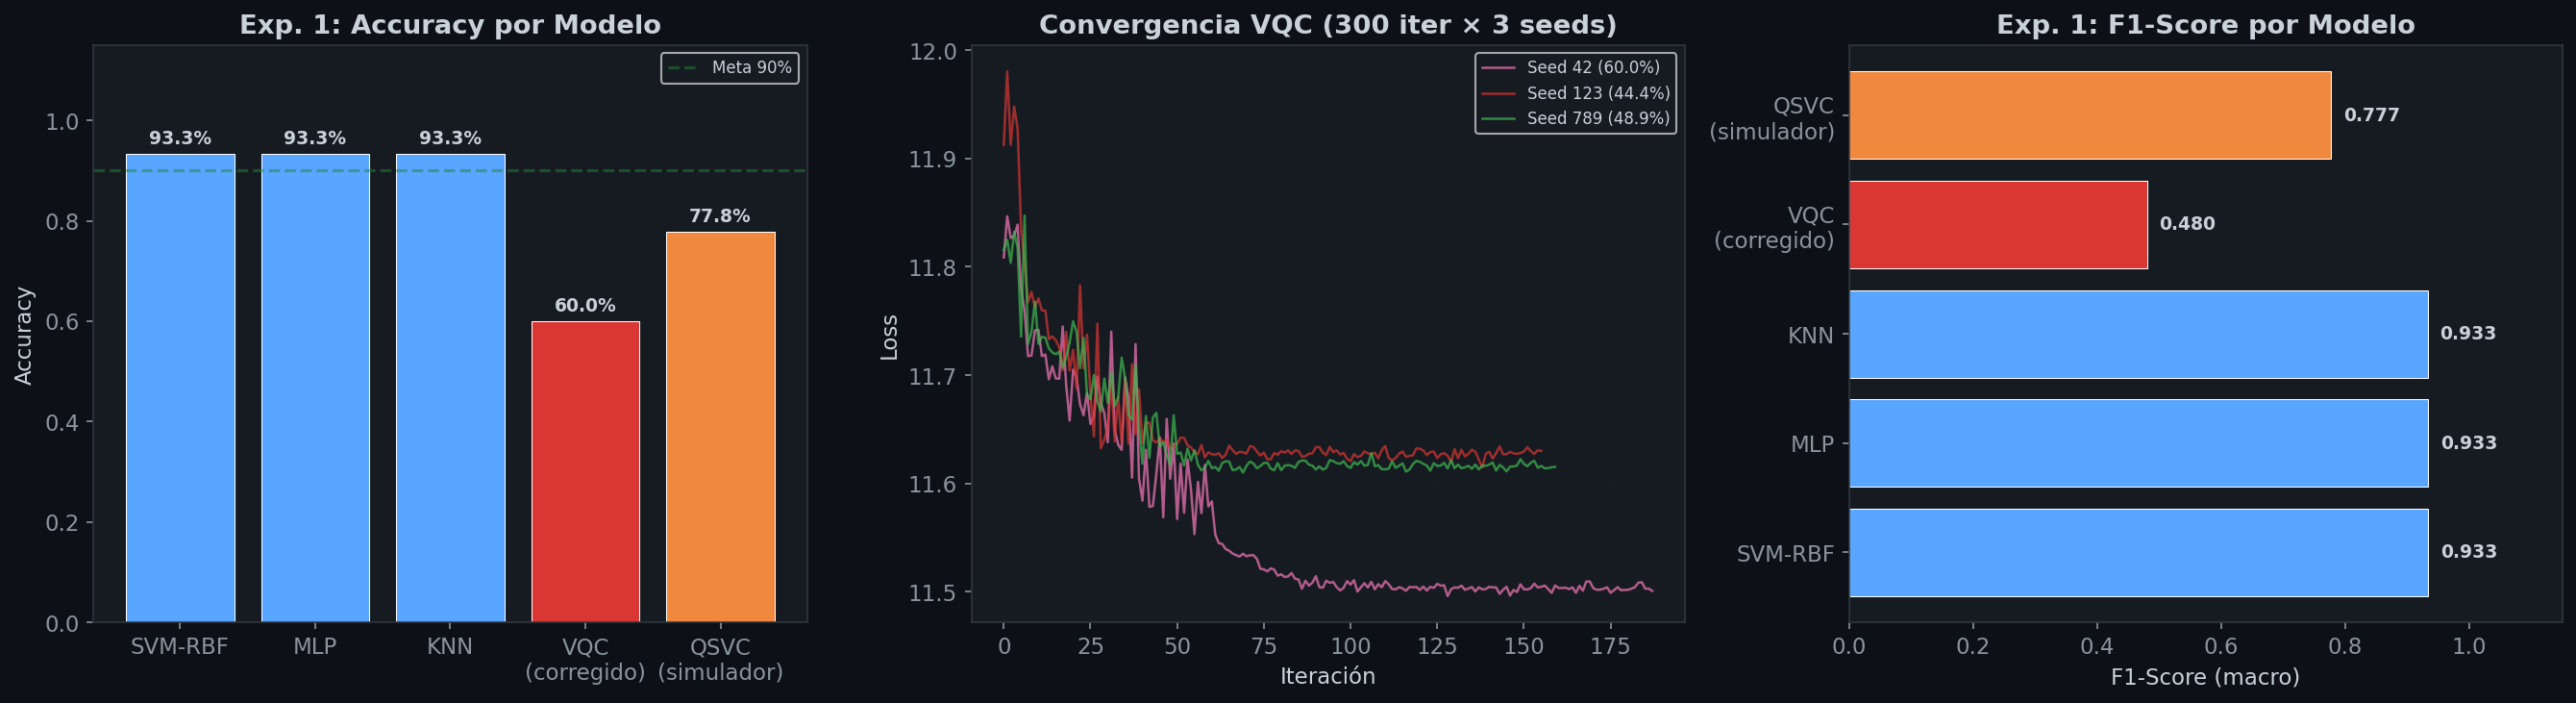
\includegraphics[width=\linewidth]{graficos/exp1_baseline_corregido.png}
    \caption{Accuracy del VQC optimizado frente a la frontera clásica (SVM 93.33\%).}
    \label{fig:baseline}
\end{figure}

\subsection{Control de calidad del hardware: fidelidad del estado de Bell}
Como control independiente de la cadena de descomposición, se preparó el estado $|\Phi^+\rangle$ (Figura~\ref{fig:bell_circuit}) en \texttt{ibm\_fez}, obteniendo una \textbf{fidelidad de 0.9834} (Figura~\ref{fig:bell}). Este resultado confirma que el procesador tiene alta calidad para operaciones básicas de entrelazamiento, lo que descarta que la degradación del kernel --reportada más adelante-- se deba a un hardware defectuoso en general.

\begin{figure}[t]
    \centering
    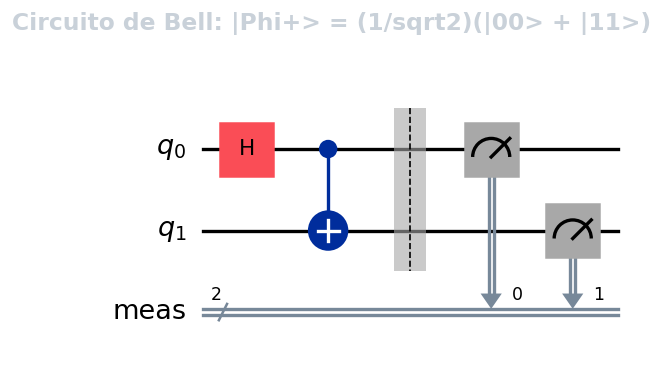
\includegraphics[width=0.85\linewidth]{graficos/vis_bell_circuit.png}
    \caption{Circuito de Bell: compuerta Hadamard sobre $q_0$ seguida de CNOT($q_0$, $q_1$), que genera el estado $|\Phi^+\rangle = \frac{1}{\sqrt{2}}(|00\rangle + |11\rangle)$.}
    \label{fig:bell_circuit}
\end{figure}

\begin{figure}[t]
    \centering
    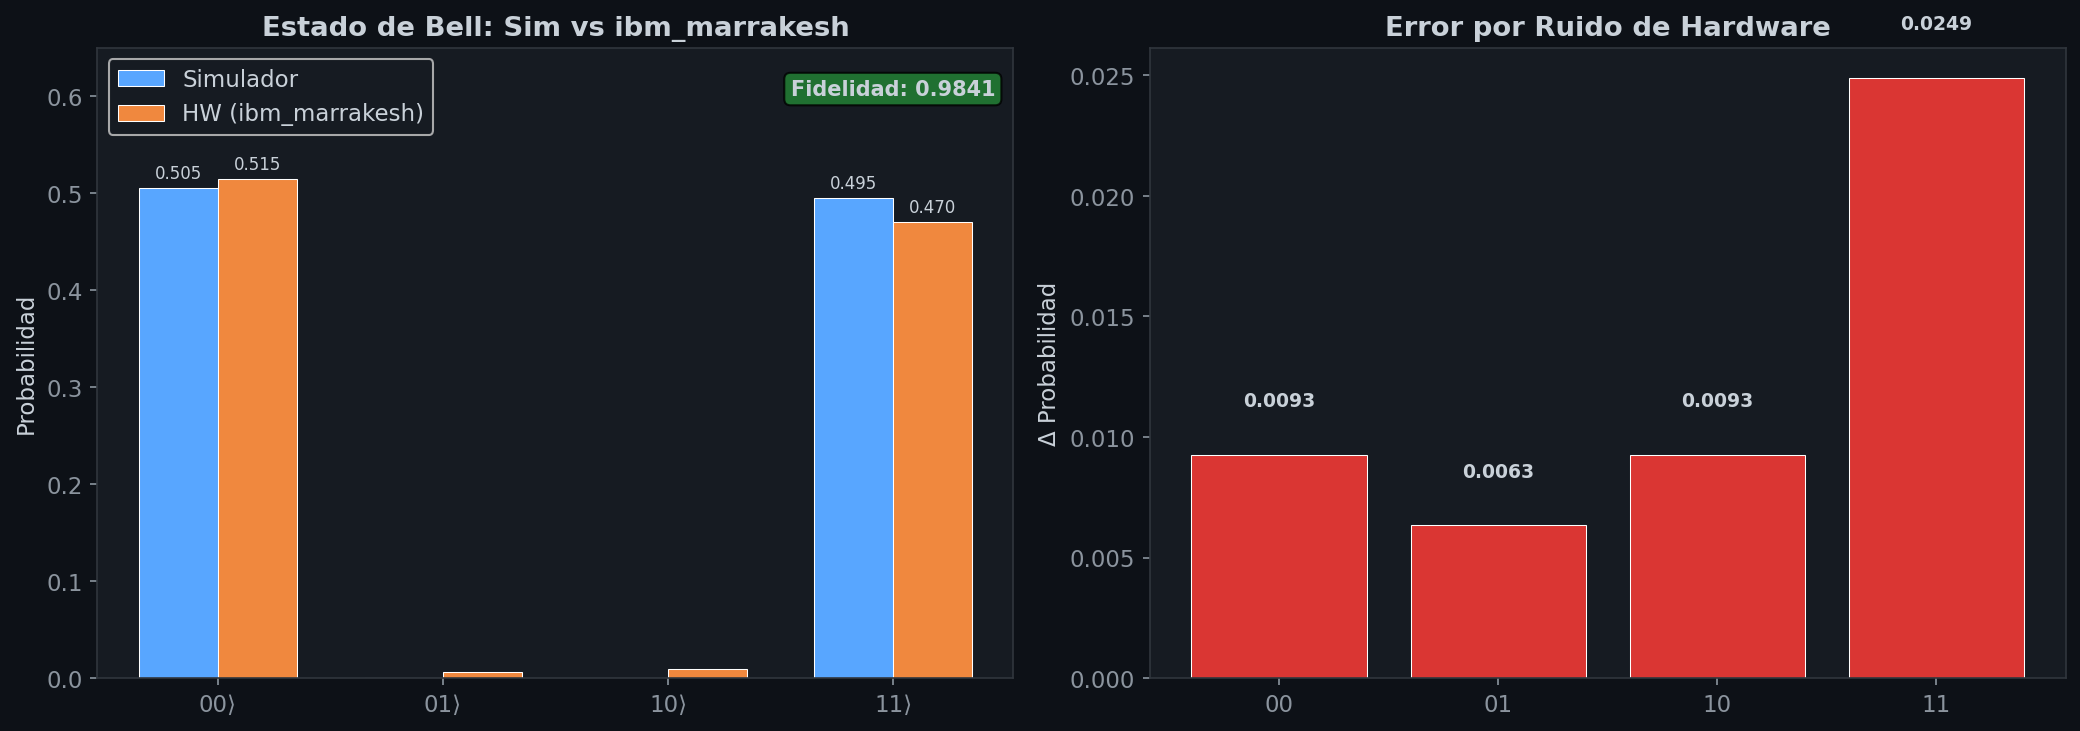
\includegraphics[width=\linewidth]{graficos/exp2_bell_state.png}
    \caption{Distribuciones de probabilidad, \textit{Statevector} vs. \texttt{ibm\_fez}, para el estado de Bell (fidelidad 0.9834).}
    \label{fig:bell}
\end{figure}

\subsection{Cadena de descomposición: QSVC en los tres puntos}
El kernel cuántico se calculó mediante el circuito \textit{compute-uncompute} (Figura~\ref{fig:kernel_circuit}): $K(\mathbf{x}_i,\mathbf{x}_j)=|\langle 0^n|U_\phi^\dagger(\mathbf{x}_j)\,U_\phi(\mathbf{x}_i)|0^n\rangle|^2$.

\begin{figure}[t]
    \centering
    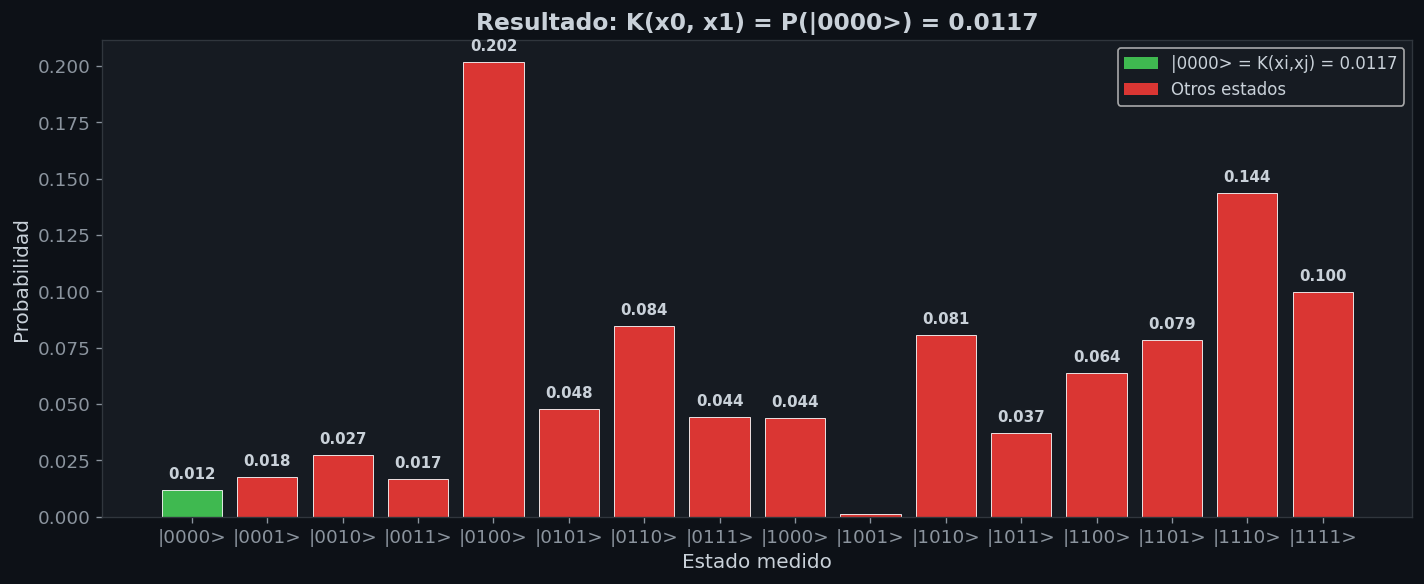
\includegraphics[width=\linewidth]{graficos/vis6_compute_uncompute_2.png}
    \caption{Circuito \textit{compute-uncompute} para el cálculo del kernel cuántico con datos reales de Iris.}
    \label{fig:kernel_circuit}
\end{figure}

La Tabla~\ref{tab:cadena} y la Figura~\ref{fig:qsvc_kernel} presentan el resultado central de este trabajo: la cadena de tres puntos que descompone la degradación total en sus dos causas.

\begin{table}[t]
\centering
\caption{Cadena de descomposición: QSVC en los tres puntos de medición.}
\label{tab:cadena}
\footnotesize
\begin{tabular}{@{}p{2.9cm}cp{2.9cm}@{}}
\toprule
\textbf{Punto de medición} & \textbf{Acc.} & \textbf{Efecto aislado} \\
\midrule
(1) Sim., Iris completo   & 77.78\% & capacidad base del kernel \\
(2) Sim., subset 13/9     & 33.33\% & $-$44 pp: escasez muestral \\
(3) HW \texttt{ibm\_fez}, subset 13/9 & 11.11\% & $-$22 pp: ruido de hardware \\
\bottomrule
\end{tabular}
\end{table}

El paso (1)$\to$(2) mantiene fijo el entorno (simulador) y solo reduce el tamaño de la muestra, aislando un efecto \emph{puro} de escasez muestral de $-$44 puntos porcentuales. El paso (2)$\to$(3) mantiene fijo el subconjunto y solo cambia el entorno de ejecución, aislando un efecto \emph{puro} de ruido de hardware de $-$22 puntos porcentuales adicionales --equivalente a clasificar correctamente solo 1 de 9 muestras de prueba--.

\begin{figure}[t]
    \centering
    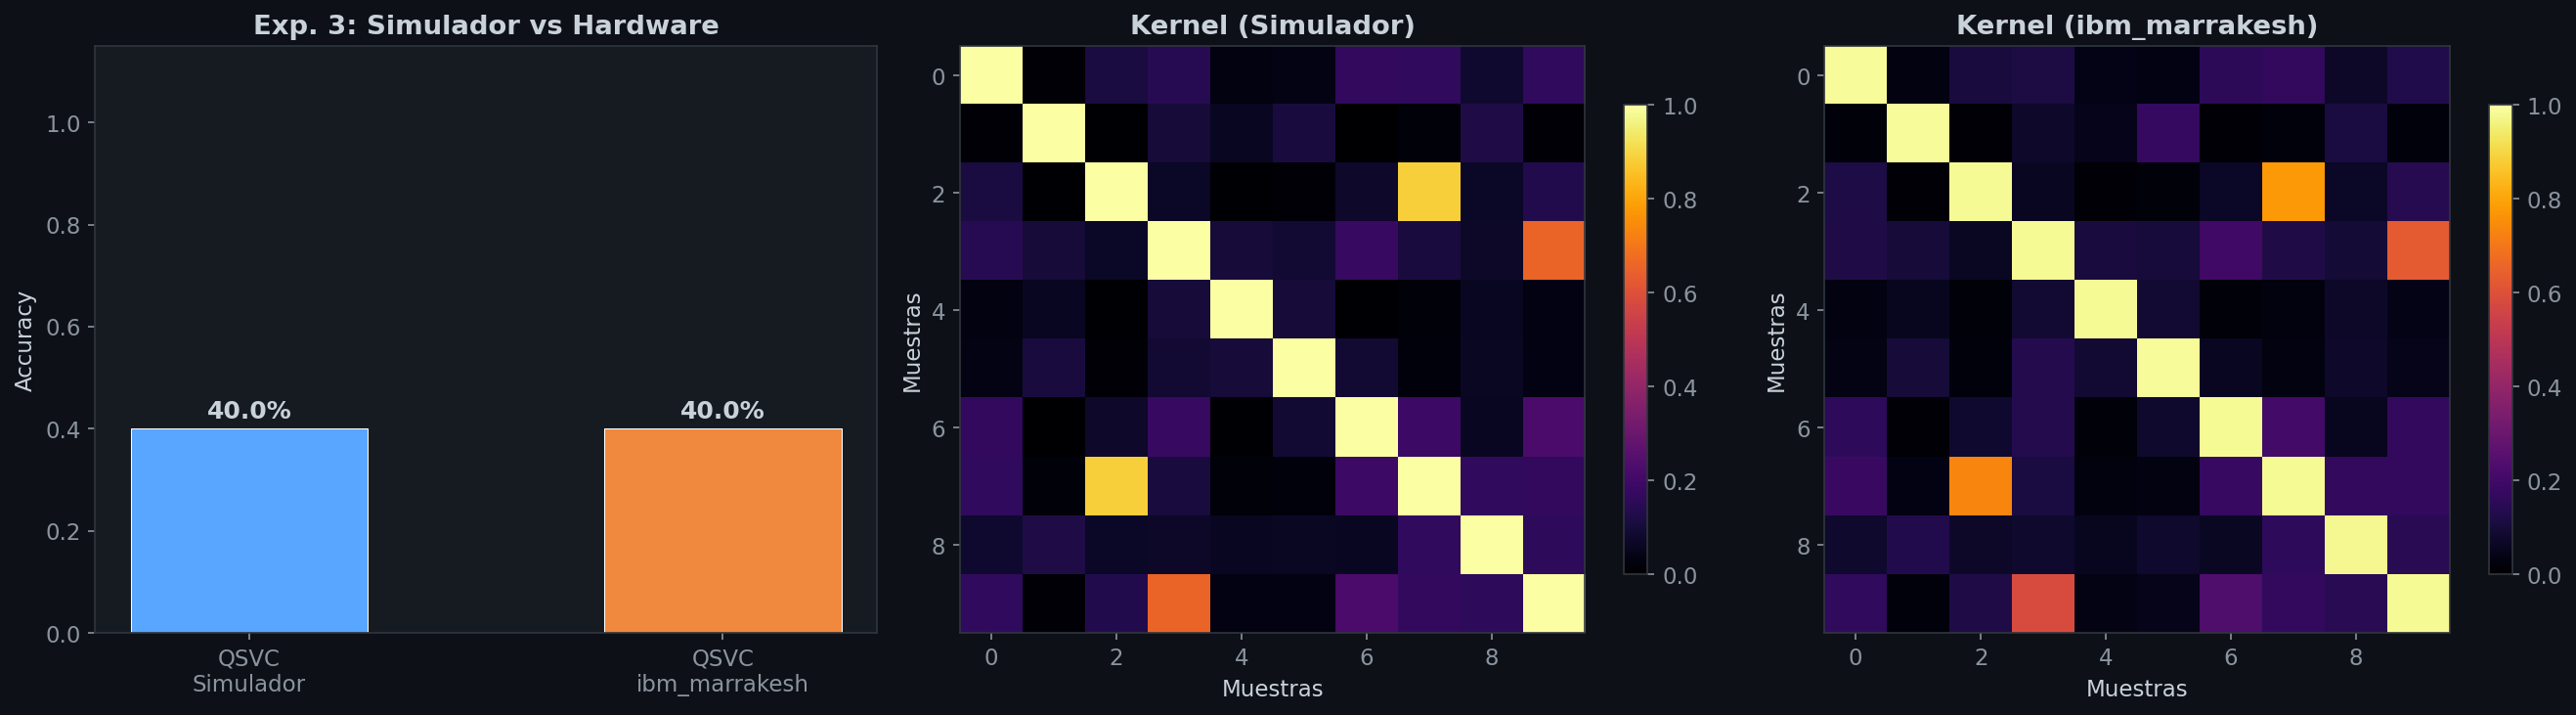
\includegraphics[width=\linewidth]{graficos/exp3_qsvc_hw_vs_sim.png}
    \caption{Matrices de similitud del kernel cuántico y accuracy comparado entre simulador (33.33\%) y hardware real (11.11\%) sobre el mismo subconjunto.}
    \label{fig:qsvc_kernel}
\end{figure}

\subsection{Mitigación TREX}
La aplicación de TREX mantuvo el accuracy invariable en \textbf{11.11\,\%}, idéntico al escenario sin mitigación (Tabla~\ref{tab:qsvc_hw}), evidenciando que la corrección de lectura no recupera información ya perdida por ruido de compuerta acumulado. La Figura~\ref{fig:trex} muestra que el error absoluto del kernel respecto al simulador ideal ($|K_{\text{sim}}-K_{\text{hw}}|$) prácticamente no se reduce con TREX activado.

\begin{figure}[t]
    \centering
    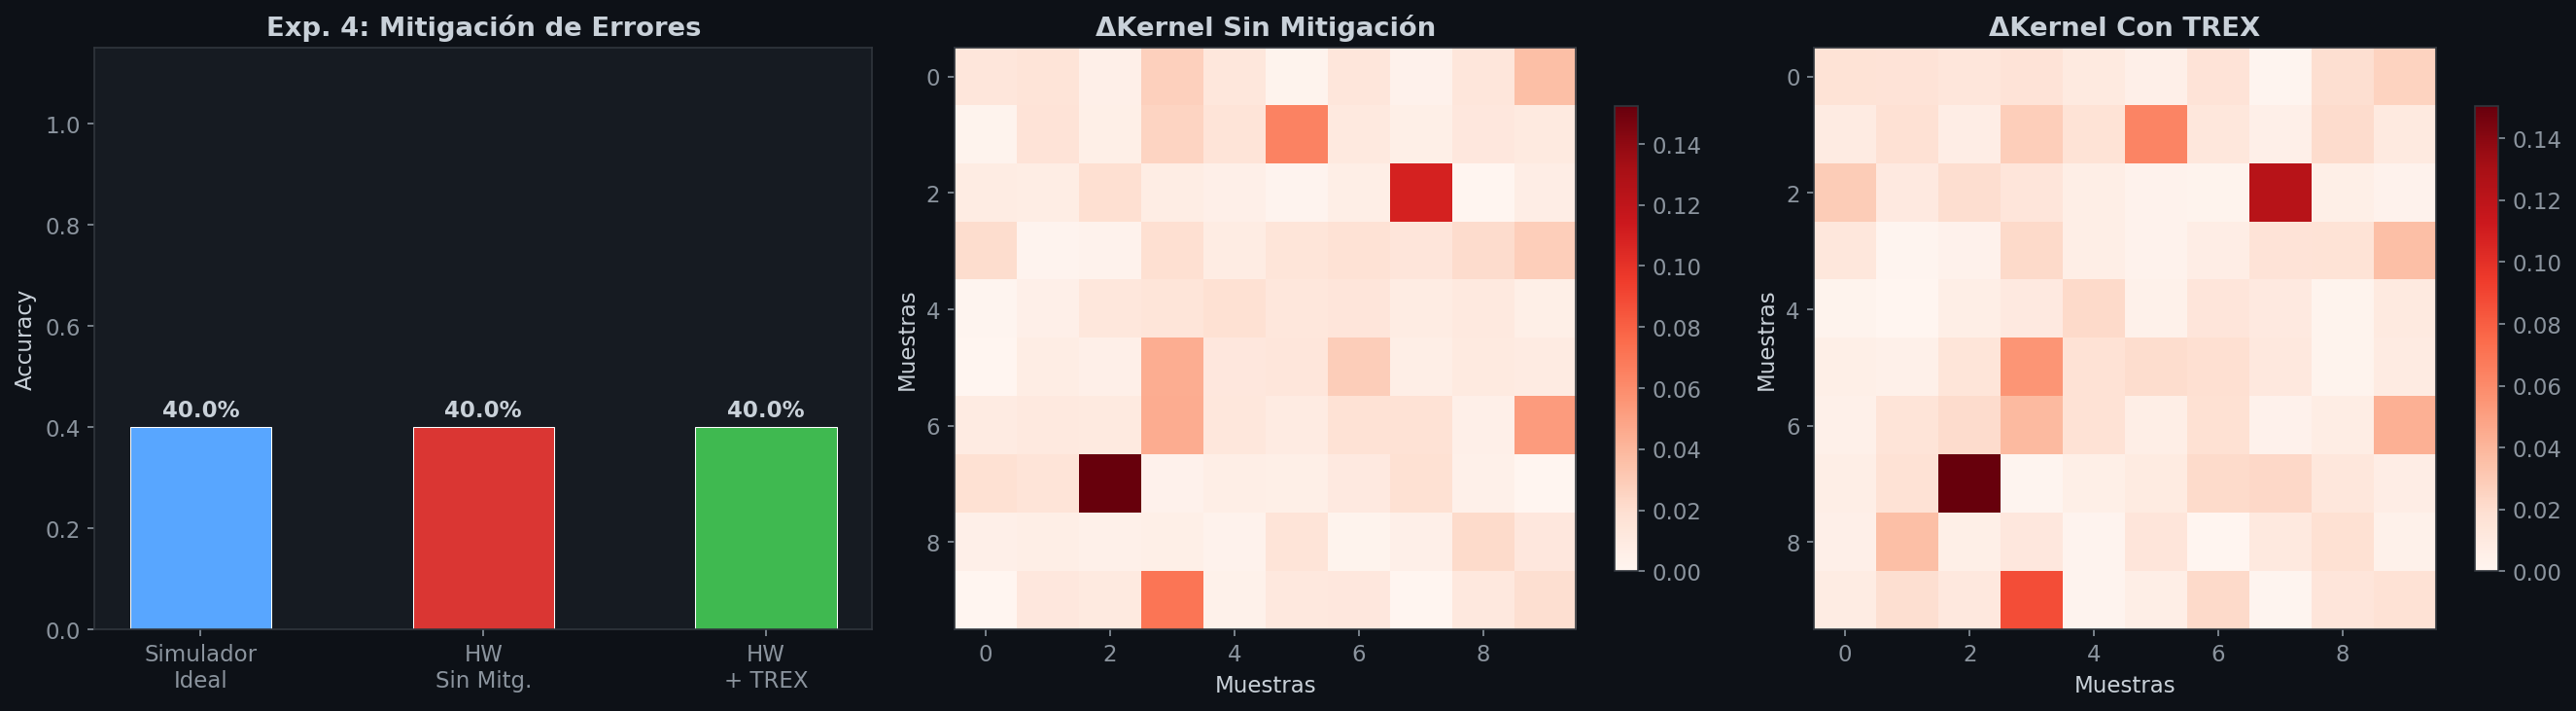
\includegraphics[width=\linewidth]{graficos/exp4_error_mitigation.png}
    \caption{Accuracy y matrices de error del kernel ($|K_{\text{sim}}-K_{\text{hw}}|$) sin mitigación vs. con TREX: el patrón de error es prácticamente idéntico en ambos casos.}
    \label{fig:trex}
\end{figure}

\begin{table}[t]
\centering
\caption{QSVC en hardware: sin mitigación vs. con TREX.}
\label{tab:qsvc_hw}
\small
\begin{tabular}{@{}lccc@{}}
\toprule
\textbf{Escenario} & \textbf{Accuracy} & \textbf{F1 (macro)} & \textbf{Tiempo QPU} \\
\midrule
HW sin mitigación & 11.11\% & 0.111 & 182s \\
HW + TREX         & 11.11\% & 0.111 & 207s \\
\bottomrule
\end{tabular}
\end{table}

\subsection{MNIST binario en hardware}
La Tabla~\ref{tab:mnist} y la Figura~\ref{fig:mnist} muestran que, de forma atípica, el hardware (88.89\,\%) superó al simulador (77.78\,\%) en la tarea binaria MNIST.

\begin{table}[t]
\centering
\caption{Resultados MNIST: clásico, simulador y hardware.}
\label{tab:mnist}
\small
\begin{tabular}{@{}lccc@{}}
\toprule
\textbf{Modelo} & \textbf{Accuracy} & \textbf{F1} & \textbf{Tiempo} \\
\midrule
SVM-RBF clásico       & 100.00\% & 1.000 & 0.01s \\
QSVC simulador          & 77.78\%  & 0.775 & 0.43s \\
QSVC hardware (\texttt{ibm\_fez}) & 88.89\% & 0.889 & 205s \\
\bottomrule
\end{tabular}
\end{table}

\begin{figure}[t]
    \centering
    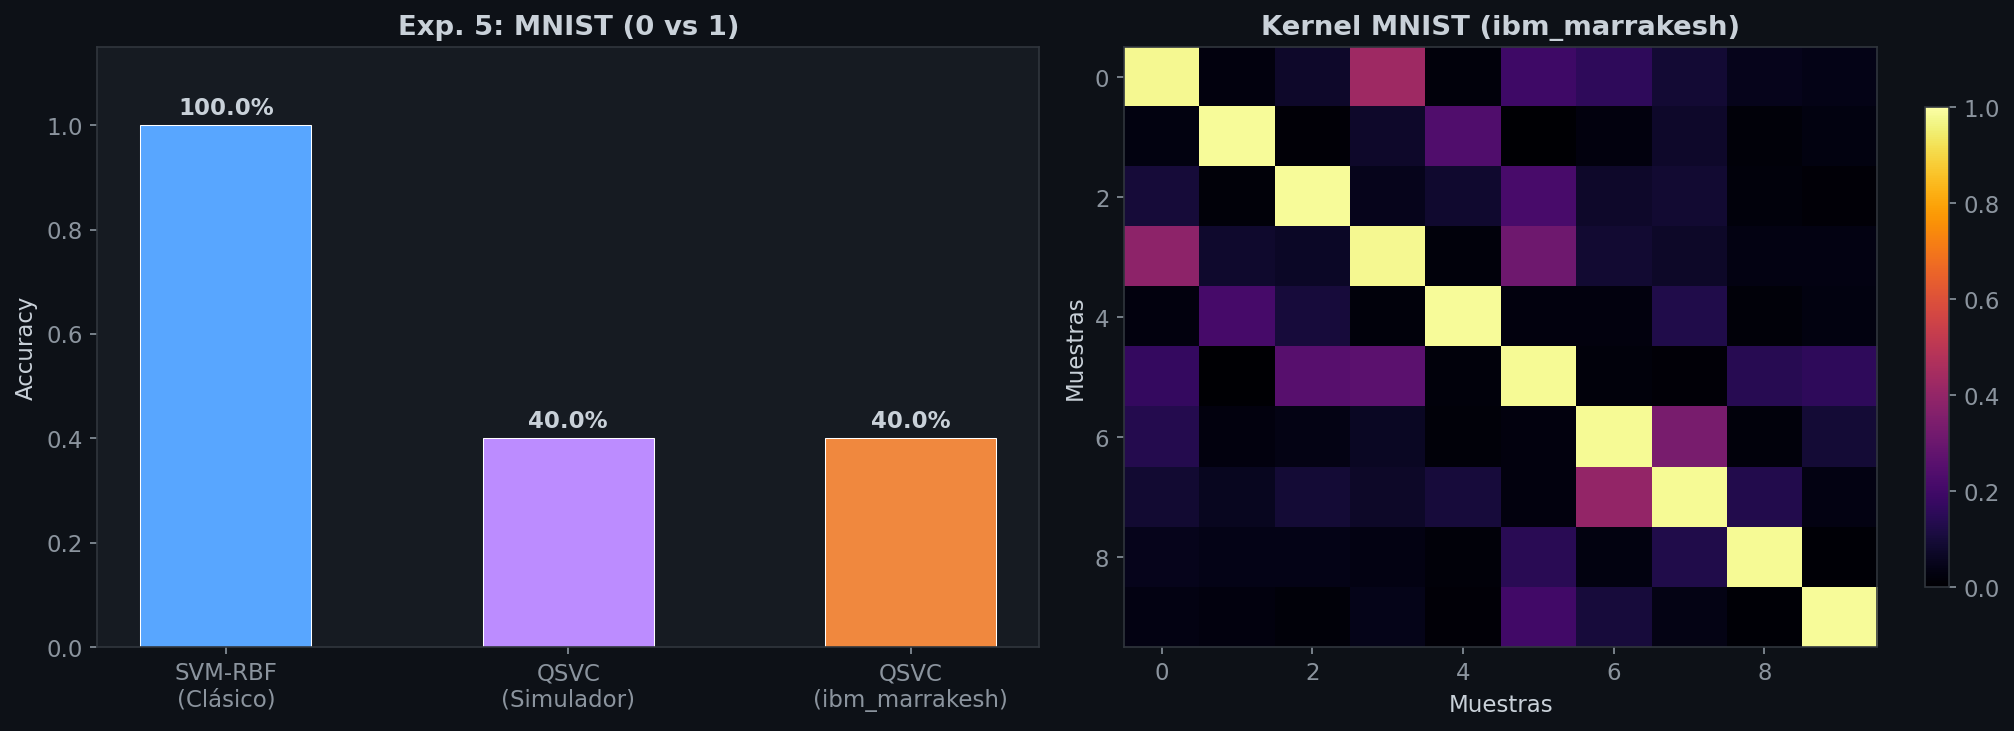
\includegraphics[width=\linewidth]{graficos/exp5_mnist_hardware.png}
    \caption{Desempeño comparativo en clasificación binaria MNIST (0 vs. 1), reducido a 4D vía PCA.}
    \label{fig:mnist}
\end{figure}

\subsection{Resumen comparativo}
La Figura~\ref{fig:radar} sintetiza todos los escenarios evaluados en un espectro radial de \textit{accuracy} y F1-\textit{score}.

\begin{figure}[t]
    \centering
    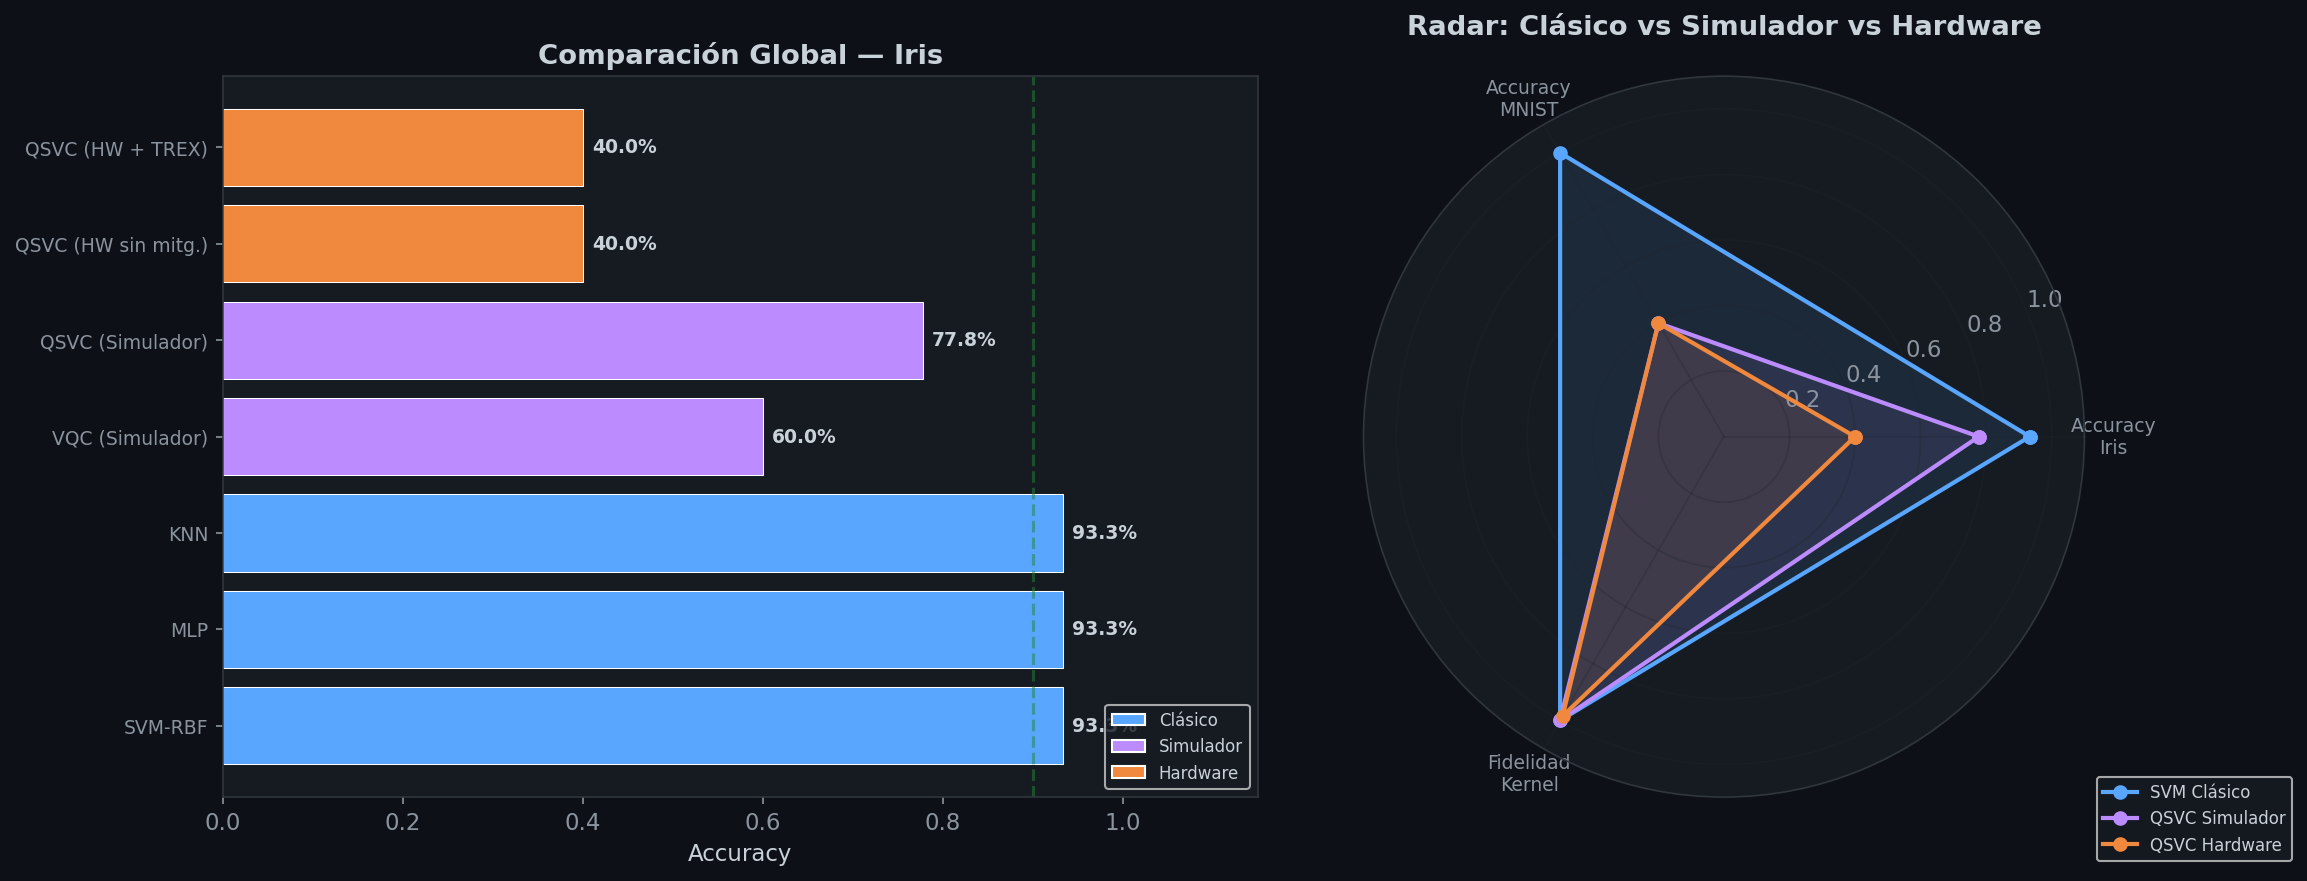
\includegraphics[width=\linewidth]{graficos/resumen_final_radar.png}
    \caption{Radar de rendimiento: accuracy y F1 (macro) para todos los escenarios evaluados.}
    \label{fig:radar}
\end{figure}

\section{Discusión}
\label{sec:discusion}

\subsection{La descomposición dual: interpretación causal y sus límites}
El hallazgo central de este trabajo es que la cadena de tres puntos permite atribuir, con precisión, cada salto de \textit{accuracy} a una causa específica en lugar de reportar un número opaco de degradación. La caída de 77.78\,\% a 33.33\,\% ($-$44 pp) al reducir el dataset de 105 a 13 muestras de entrenamiento, manteniendo fijo el entorno de simulación, se atribuye a la insuficiencia de densidad topológica: un clasificador SVM embebido en un espacio de Hilbert de dimensión $2^4=16$ no dispone de suficientes vectores de soporte para trazar fronteras de decisión generalizables \cite{schuld2019}. Sobre esta base ya degradada, mantener fijo el subconjunto y solo cambiar el entorno a hardware real redujo el accuracy adicionalmente a 11.11\,\% ($-$22 pp), lo que constituye evidencia --dentro de este experimento controlado-- de que el ruido NISQ contribuye de forma independiente a la degradación, más allá de lo explicado por la escasez de datos.

Es importante encuadrar esta magnitud con honestidad: con 9 muestras de prueba, cada una vale $\pm$11.1\,\% de \textit{accuracy}, de modo que el salto de $-$22 pp equivale a 2 muestras y proviene de \textbf{una sola corrida} en hardware. La contribución de este trabajo no es la magnitud puntual --que requeriría repeticiones para estimar su varianza-- sino el \textbf{protocolo de descomposición} en sí: el diseño escalonado (mismo kernel, mismo subconjunto, solo cambia el entorno) es lo que permite, en principio, atribuir causas de forma reproducible, independientemente del tamaño exacto del efecto medido en una ejecución particular.

\subsection{Por qué TREX falla sobre un kernel ya colapsado}
El experimento arroja un contraste que ilumina el mecanismo de fallo: la fidelidad del estado de Bell en \texttt{ibm\_fez} fue de \textbf{0.9834} --el hardware es objetivamente bueno para entrelazamiento básico de 2 qubits-- y sin embargo el kernel QSVC colapsó a 11.11\,\% y \textbf{TREX no lo mejoró en absoluto}. La explicación es que TREX, por diseño, corrige asimetrías sistemáticas de \emph{lectura} (errores SPAM) \cite{vandenberg2022}, pero el circuito \textit{compute-uncompute} $U_\phi(\mathbf{x}_i)\cdot U_\phi^\dagger(\mathbf{x}_j)$ es sustancialmente más profundo que el circuito de Bell, y acumula ruido de \emph{compuerta} durante su ejecución, agravado por la concentración exponencial que sufren los kernels cuánticos al escalar \cite{thanasilp2024}. La información ya se pierde \emph{antes} de la medición, de modo que corregir la lectura no puede recuperar nada. Esta hipótesis mecanística es consistente con el contraste de fidelidades observado, aunque --al no haberse ejecutado en este trabajo un experimento de \textit{Zero Noise Extrapolation} (ZNE) \cite{temme2017} que opere directamente sobre el ruido de compuerta-- queda como una interpretación respaldada por evidencia indirecta y no como una prueba directa; se plantea explícitamente como trabajo futuro en la Sección~\ref{sec:conclusiones}. La lección práctica es que TREX no debe asumirse como remedio general para kernels cuánticos degradados: su efectividad depende de que la causa dominante del error sea de lectura y no de acumulación de ruido de compuerta.

\subsection{El caso atípico de MNIST como artefacto de reproducibilidad}
Que el hardware (88.89\,\%) superara al simulador (77.78\,\%) en MNIST no debe interpretarse como ventaja cuántica: con solo 9 muestras de prueba, cada clasificación individual representa $\sim$11.1\,\% del accuracy, y la tarea binaria (frente a las 3 clases de Iris) eleva la probabilidad base de acierto por azar. Las perturbaciones estocásticas del ruido cuántico pueden, en problemas de baja complejidad, actuar como una forma de regularización implícita que favorece por azar la separabilidad \cite{huang2021}; con datasets más grandes es esperable que el simulador supere sistemáticamente al hardware ruidoso. Este resultado es, en sí mismo, una advertencia de reproducibilidad relevante para la comunidad que --como la mayoría de estudiantes e investigadores sin acceso premium-- opera bajo el mismo régimen de cuotas gratuitas: bajo baja resolución muestral, un solo resultado favorable al hardware puede malinterpretarse como evidencia de ventaja cuántica cuando en realidad es ruido estadístico.

\subsection{Brecha cuántico-clásica}
Los modelos clásicos mantuvieron 93.33\,\% uniforme sobre Iris completo, frente al mejor resultado cuántico de 60.00\,\% (VQC). Esta brecha de 33 puntos porcentuales es consistente con los hallazgos a gran escala de Bowles \textit{et al.} \cite{bowles2024}, reforzando que los modelos cuánticos actuales no ofrecen ventaja competitiva frente a algoritmos clásicos bien calibrados bajo las restricciones operacionales de la era NISQ. Como limitación general, este estudio opera sobre un único procesador (\texttt{ibm\_fez}) y un subconjunto muestral extremadamente reducido por razones de cuota, por lo que la generalización de las magnitudes exactas de degradación a otros \textit{backends} o tamaños muestrales requiere validación adicional; el protocolo de descomposición, sin embargo, es directamente reutilizable en esos escenarios.

\section{Conclusiones y Trabajo Futuro}
\label{sec:conclusiones}

Este trabajo propuso y validó un protocolo de descomposición de tres puntos que separa, dentro de un mismo experimento controlado, la degradación de un clasificador de kernel cuántico (QSVC) atribuible a la escasez muestral de la atribuible al ruido de hardware NISQ. El protocolo aisló un efecto puro de escasez muestral de $-$44 puntos porcentuales (de 77.78\,\% a 33.33\,\% en simulador) y un efecto puro adicional de ruido de hardware de $-$22 puntos porcentuales (hasta 11.11\,\% en \texttt{ibm\_fez}). La verificación del estado de Bell (fidelidad 0.9834) confirmó la buena calidad general del hardware, lo que --junto con la ineficacia de TREX-- sustenta la hipótesis de que el kernel se degrada por acumulación de ruido de compuerta durante el circuito \textit{compute-uncompute}, y no por errores de lectura. El VQC optimizado (300 iteraciones COBYLA) alcanzó un máximo de 60.00\,\% de accuracy, aún 33 puntos porcentuales por debajo de los clásicos SVM-RBF, MLP y KNN (93.33\,\%), y el aparente mejor desempeño del hardware sobre el simulador en MNIST binario se identificó como un artefacto estadístico de baja resolución muestral bajo el régimen de acceso gratuito, no como evidencia de ventaja cuántica.

En respuesta a los objetivos planteados: (i) el protocolo de descomposición funciona y es reproducible con los recursos de una cuenta gratuita de IBM Quantum; (ii) TREX es insuficiente frente a degradación dominada por ruido de compuerta, y se requieren técnicas complementarias a nivel de compuerta; y (iii) los resultados favorables al hardware bajo baja resolución muestral deben interpretarse con cautela explícita antes de atribuirlos a ventaja cuántica. Como trabajo futuro se plantean tres líneas: (i) ejecutar un experimento de \textit{Zero Noise Extrapolation} (ZNE) \cite{temme2017} sobre el mismo kernel colapsado para probar directamente la hipótesis de daño a nivel de compuerta, en lugar de inferirla del contraste de fidelidades; (ii) migrar a planes de acceso premium de IBM Quantum que permitan evaluar el kernel físico sobre el conjunto de datos completo, aislando el efecto del ruido sin la restricción muestral y repitiendo cada punto de la cadena para estimar su varianza; y (iii) replicar el protocolo de descomposición sobre una fracción del \textit{benchmark} de Bowles \textit{et al.} \cite{bowles2024}, para determinar si la relación $-$44~pp/$-$22~pp observada aquí se generaliza a otros datasets y \textit{backends} \cite{huang2021,biamonte2017}.

\bibliographystyle{IEEEtran}
\bibliography{contenido/bibliografia}

\end{document}
